\documentclass[10pt]{article}
\usepackage{icmlko}

\icmlmeta{IP 파운데이션 월드모델}{178}{유명한 쪽으로 틀린다, 그런데 맞을 때도 그렇다}{노트 177의 첫 줄대로 세 도메인에 한국어 위키를 댔다. 아이돌 덮음이 0에서 79\%가 됐는데 판은 안 움직였고, 옆에서 나온 매칭 품질 문제가 판을 움직였다 --- 다만 채택할 수 없다}

\begin{document}

\twocolumn[
\icmlheader

\begin{abstract}
노트 177이 ``도서 · 펀딩 · 아이돌은 영문 위키만 대 봤고 한국어판은 안
댔다''를 첫 줄에 남겼다. 댔다. \textbf{아이돌 덮음이 0\%에서 79\%가 된다}
--- 그룹 78건 중 66건이 문서에 붙고 43건은 데뷔 이전 90일 창에 조회수까지
있다. 예측(매칭 60\% · 조회 25\%)보다 훨씬 높다. 데뷔 전에 문서가 생기기
때문이다. 도서는 21\%, \textbf{펀딩은 0.3\%} --- 노트 177이 ``이 셋도
0\%는 아닐 것''이라 적었는데 펀딩은 정말로 0이다. 크라우드펀딩 프로젝트
제목은 문장이라 위키 문서가 있을 수 없다. \textbf{그런데 판이 안
움직인다} --- 세 도메인을 다 넣어 $+$0.0010($t{=}0.55$)이다. \textbf{수집을
0에서 79\%로 올려도 판정치는 모른 척한다.} 그러다 옆에서 둘을 주웠다.
① \textbf{버그} --- MediaWiki 는 제목에 \texttt{<>[]|\{\}\#} 가 있으면
\texttt{missing} 이 아니라 \texttt{invalid} 을 주는데 \texttt{title} 은
우리가 보낸 문자열 그대로다. 그것을 문서로 받았다(351건). 다행히
\textbf{그중 조회수가 붙은 것은 0건}이라 축은 한 번도 안 더러웠다.
② \textbf{정규식이 한국어를 몰랐다} --- \texttt{franchise()} 가 ``season
3''은 아는데 ``14기''는 모른다. 그래서 애니 207건이 검색으로 새어 겹침
포함(0.8)으로 붙었다 --- \emph{옳은} 문서에 붙었는데 점수만 낮았다.
고치니 애니의 포함 비중이 47\%에서 13\%로 떨어진다. 그다음 물었다:
포함 매칭을 버리면? \textbf{판이 $+$0.0050 오른다($t{=}2.0$).} 내 예측은
반대였다. \textbf{그런데 채택 안 한다} --- 갈라 보니 게임 $+$0.034 대
세계애니 \textbf{$-$0.023}으로 부호가 갈리고, 손으로 세면 세계애니의 포함
매칭은 7/7 옳다. 마지막으로 매력적인 진단 하나를 죽였다. 포함 매칭은
조회수가 \textbf{$+$0.83 더 높다}($p{=}2\times10^{-16}$) --- 노트 177과
같은 방향이라 ``부풀림 $=$ 오매칭''으로 읽고 싶다. \textbf{아니다.}
도메인별로 부풀림과 판 이득이 \textbf{반대로 붙는다}($\rho{=}-0.66$) ---
제일 많이 부푼 세계애니가 버리면 제일 많이 잃는다. \textbf{옳은 프랜차이즈
매칭도 똑같이 부푼다.}
\end{abstract}
]

\begin{figure*}[t]
\centering
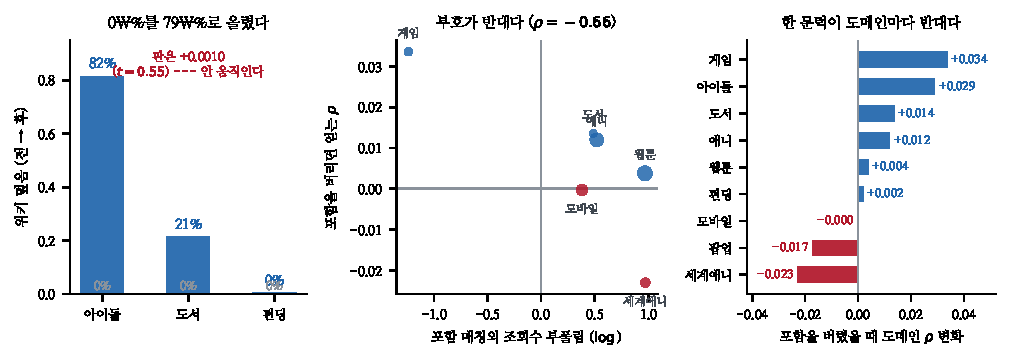
\includegraphics[width=\textwidth]{figs/famous.pdf}
\caption{왼쪽 --- 0\%를 79\%로 올렸는데 판은 그대로다. 가운데 --- 부풀림과
판 이득이 반대로 붙는다. 오른쪽 --- 한 문턱이 도메인마다 반대다.}
\end{figure*}

\section{한국어 위키를 댔다}

\begin{table}[t]
\centering\tsize
\caption{닻은 아이돌 데뷔일 · 도서 출간일 · 펀딩 시작일. 창은 그 이전 90일.}
\begin{tabular}{lrrrr}
\toprule
& 대상 & 문서 & 창에 조회수 & 덮음 \\
\midrule
\textbf{아이돌} & 78 & 66 (85\%) & \textbf{43 (55\%)} & \textbf{79\%} \\
도서 & 351 & 90 (26\%) & 82 (23\%) & 21\% \\
\textbf{펀딩} & 399 & \textbf{1} & \textbf{1} & \textbf{0.3\%} \\
\bottomrule
\end{tabular}
\end{table}

\claimx{\textbf{아이돌이 예측을 크게 넘었다}(매칭 60\% 예측에 85\%, 조회
25\% 예측에 55\%). 창이 \emph{데뷔 이전}이라 문서가 아직 없을 줄
알았다.}{까닭은 데뷔 방식이다 --- 서바이벌 · 티저로 몇 달 전에 공개되고
그때 문서가 생긴다. \textbf{그래서 데뷔 전 조회수가 실제로 존재한다.}}

\claimx{\textbf{펀딩은 정말로 0이다.} 노트 177이 ``팝업이 한국어판으로
60\%를 얻었으니 이 셋도 0\%는 아닐 것''이라 적었는데 \textbf{그 예측은
펀딩에서 틀렸다.}}{까닭이 분명하다 --- ``내 취향 와인을 찾기 위해,
`와인 테이스팅 다이어리'\,''는 IP 이름이 아니라 문장이다.
\textbf{펀딩에는 IP 가 없다.}}

\section{그런데 판이 안 움직인다}

\begin{table}[t]
\centering\tsize
\caption{세 도메인을 축 지도에 넣으면. 짝 부트스트랩 400회.}
\begin{tabular}{lrrrl}
\toprule
& 기존 6 & 새 3 추가 & 차 & \\
\midrule
F18 배깅 & .4516 & .4526 & $+$.0010 & $t{=}0.55$ \\
F6 능형 & .3707 & .3710 & $+$.0003 & $t{=}0.23$ \\
\bottomrule
\end{tabular}
\end{table}

\claimx{\textbf{덮음을 0에서 79\%로 올려도 판은 모른 척한다.} 아이돌
유보가 25건뿐이고(판의 1\%) 도서 163건은 덮음이 21\%다.}{내 예측이
맞았다($|\Delta| < 0.005$). \textbf{그런데 맞아서 기쁜 예측이
아니다} --- 노트 176이 ``자료를 더 모으면 판이 내려갈 수 있다''를 세웠고
이번엔 ``올려도 안 움직인다''다. \textbf{둘 다 판정치가 수집에 둔하다는
말이다.}}

\section{옆에서 주운 것 둘}

\begin{table}[t]
\centering\tsize
\caption{\texttt{invalid} 를 문서로 받은 레코드.}
\begin{tabular}{lrr}
\toprule
& 건수 & 조회수 붙은 것 \\
\midrule
펀딩 & 166 & 0 \\
애니 & 157 & 0 \\
나머지 넷 & 28 & 0 \\
\midrule
\textbf{합} & \textbf{351} & \textbf{0} \\
고친 뒤 되찾음 & & 6 \\
\bottomrule
\end{tabular}
\end{table}

\claimx{\textbf{버그는 진짜인데 값이 없었다.} 351건 전부 조회수가 0이라
축은 한 번도 안 더러웠고, 고쳐서 되찾은 것도 6건뿐이다.}{그래도 고칠
값은 있었다 --- 가짜 문서가 붙으면 프랜차이즈 · 검색 되돌리기를 건너뛴다.
\textbf{여섯 번째 측정 아티팩트인데 처음으로 표제를 안 뒤집었다.}}

\begin{table}[t]
\centering\tsize
\caption{\texttt{franchise()} 에 한국어 속편 표기를 넣으면.}
\begin{tabular}{lrr}
\toprule
& 전 & 후 \\
\midrule
애니 포함 매칭 비중 & 47.4\% & \textbf{12.8\%} \\
애니 프랜차이즈 매칭 & 0 & \textbf{205} \\
전체 포함 비중 & 24.4\% & 18.1\% \\
\midrule
\textbf{판(문턱 0)} & .4495 & \textbf{.4495} \\
\bottomrule
\end{tabular}
\end{table}

\claimx{\textbf{판이 한 자리도 안 움직인다.} 검색 대체가 이미 같은 문서를
찾고 있었다 --- ``(더빙) 명탐정 코난 14기''가 겹침 포함으로 ``명탐정
코난''에 옳게 붙어 있었다. 바뀌는 것은 \emph{점수}뿐이다.}{그러니 이건
성능 고침이 아니라 \textbf{품질 표시 고침}이다. 옳게 붙은 것에 옳은
점수를 준다.}

\section{문턱은 판을 올리는데 채택 못 한다}

\begin{table}[t]
\centering\tsize
\caption{매칭 점수 문턱별 판 $\rho$.}
\begin{tabular}{lrr}
\toprule
& F18 배깅 & F6 능형 \\
\midrule
현행 (0.8 포함) & .4495 & .3668 \\
\textbf{포함 버림 ($\ge$0.9)} & \textbf{.4543} & .3687 \\
정확만 ($\ge$1.0) & .4508 & \textbf{.3706} \\
\midrule
버림 $-$ 현행 & $+$.0050 & $+$.0020 \\
& $t{=}1.98$ & $t{=}1.20$ \\
\bottomrule
\end{tabular}
\end{table}

\claimx{\textbf{내 예측이 방향부터 틀렸다.} ``마스크가 신호를 나르니
버리면 잃는다''로 $-$0.005$\sim$$-$0.020 을 적었는데 $+$0.0050
이다.}{까닭은 노트 176과 이 노트의 차이에 있다 --- 노트 176이 지운 것은
\emph{빈칸}이고 여기서 지우는 것은 \emph{틀린 값}이다. \textbf{빈칸은
바닥에 앉고 틀린 값은 아무 데나 앉는다.}}

\begin{table}[t]
\centering\tsize
\caption{그런데 갈라 보면 부호가 갈린다(F18).}
\begin{tabular}{lrrl}
\toprule
& n & 버림 $-$ 현행 & 손으로 본 정확도 \\
\midrule
\textbf{게임} & 223 & \textbf{$+$.0336} & 28 중 8 \\
애니 & 606 & $+$.0120 & --- \\
도서 & 163 & $+$.0136 & 15 중 4 \\
웹툰 & 711 & $+$.0038 & --- \\
모바일 & 441 & $-$.0003 & 7 중 6 \\
\textbf{세계애니} & 300 & \textbf{$-$.0230} & \textbf{7 중 7} \\
\bottomrule
\end{tabular}
\end{table}

\claimx{\textbf{제일 정확한 도메인이 제일 많이 잃는다.} 세계애니의 포함
매칭은 손으로 일곱을 보니 일곱이 다 옳고, 버리면 $-$0.023 이다. 게임은
스물여덟 중 여덟만 옳고 버리면 $+$0.034 다.}{\textbf{그래서 채택 안
한다.} 전역 문턱은 게임을 고치려고 세계애니를 부순다. 판을 보고 도메인별
문턱을 고르면 그게 노트 126이 잡은 그 잘못이다.}

\claimx{게임이 왜 그렇게 나쁜지는 목록에 그대로 보인다 --- \textbf{조회수
5,570,493 짜리 ``Backrooms (film)''이 인디 게임 ``Backrooms Lost
Runners''에 붙어 있다.} ``Drone racing''$\leftarrow$``Liftoff: FPV Drone
Racing'', ``Train simulator''$\leftarrow$``JR EAST Train Simulator''.}{스팀
표본은 인디가 많아 진짜 문서가 없고, 그래서 일반 명사 문서로 샌다.
세계애니의 포함 매칭은 반대로 ``Blue Archive''$\leftarrow$``Blue Archive
The Animation''처럼 \emph{같은 프랜차이즈의 부제}다.}

\section{매력적인 진단 하나를 죽였다}

\begin{table}[t]
\centering\tsize
\caption{포함 매칭의 $\log$ 조회수 부풀림.}
\begin{tabular}{lrrl}
\toprule
& 부풀림 & 판 이득 & \\
\midrule
\textbf{세계애니} & \textbf{$+$0.97} & \textbf{$-$.023} & 어긋남 \\
웹툰 & $+$0.97 & $+$.004 & \\
애니 & $+$0.52 & $+$.012 & \\
도서 & $+$0.49 & $+$.014 & \\
모바일 & $+$0.38 & $-$.000 & \\
\textbf{게임} & \textbf{$-$1.24} & \textbf{$+$.034} & 어긋남 \\
\midrule
전체 & $+$0.83 & & $p{=}2{\times}10^{-16}$ \\
\bottomrule
\end{tabular}
\end{table}

\claimx{\textbf{부풀림은 오매칭의 증거가 아니다.} 전체로는 포함 매칭이
$+$0.83 더 유명하고($p{=}2\times10^{-16}$) 노트 177과 같은 방향이라
``부풀면 틀린 것''으로 읽고 싶다. \textbf{그런데 도메인별로는 반대로
붙는다}($\rho{=}-0.66$ · $r{=}-0.81$).}{까닭이 하나다 --- 옳은 프랜차이즈
매칭도 부푼다. ``Blue Archive The Animation''을 ``Blue Archive''에 옳게
붙이면 조회수가 올라간다. \textbf{부풀림은 오매칭과 정매칭을 못 가른다.}}

\claimx{\textbf{노트 177을 한 겹 좁힌다.} 노트 177이 ``어렵게 찾은 것이
더 유명했다''를 ``매칭 난이도는 제목의 모양을 잰다''로 읽었다. 맞다 ---
그리고 \textbf{그 유명함은 옳을 때도 틀릴 때도 똑같이 나온다.}}{도메인
여섯뿐이라 $\rho{=}-0.66$ 을 세게 읽지는 않는다. \textbf{읽을 수 있는
것은 ``부풀림으로 품질을 판정할 수 없다''는 부정형이다.}}

\section{그래서 무엇을 채택하나}

\begin{table}[t]
\centering\tsize
\caption{이 사이클의 결정.}
\begin{tabular}{ll}
\toprule
\textbf{채택} & \texttt{invalid} 고침 (351건) \\
\textbf{채택} & 한국어 속편 규칙 (애니 205건 승격) \\
\textbf{채택} & 도서 · 아이돌 위키 축 ($+$.0010, 안 갈림) \\
\midrule
\textbf{안 함} & 전역 매칭 문턱 ($+$.0050 인데 부호가 갈림) \\
\textbf{안 함} & 펀딩 위키 --- 붙을 문서가 없다 \\
\bottomrule
\end{tabular}
\end{table}

\claimx{\textbf{판을 올리는 것 하나를 일부러 안 채택했다.} $+$0.0050
($t{=}2.0$)이면 이 흐름에서 큰 걸음이다 --- 노트 170의 위키 축 전체
이득이 $+$0.0096 이었다. 그래도 안 한다.}{노트 176이 ``판이 내려가는
것이 나쁜 모형을 뜻하지 않는다''를 세운 자리의 거울상이다 --- \textbf{판이
올라가는 것도 좋은 자료를 뜻하지 않는다.}}

\begin{table}[t]
\centering\tsize
\caption{남은 것.}
\begin{tabular}{ll}
\toprule
\textbf{게임} & 일반 명사 문서로 새는 것을 규칙으로 막을 수 있나 \\
아이돌 & 닻이 데뷔일이다 --- 앨범 발매일을 못 찾았다 \\
판정치 & 수집을 0$\to$79\% 올려도 안 움직이는 것이 옳은가 \\
\bottomrule
\end{tabular}
\end{table}

첫 줄이 곧바로 잴 수 있다. 게임의 오매칭은 전부 \emph{일반 명사} 문서다
--- ``물'' · ``여름'' · ``Drone racing'' · ``Train simulator''. 그 문서들은
게임이 나오기 훨씬 전부터 존재했고 조회수가 평평하다. \textbf{창 안에서
기울기가 0에 가깝고 수준이 높으면 그건 그 IP 문서가 아니다} --- 문턱
대신 그것을 규칙으로 쓰면 도메인을 안 가리고 게임만 고칠 수 있다.

\end{document}
